\documentclass[a4paper, 16pt]{article}
\usepackage[slovene]{babel}
\usepackage[utf8]{inputenc}
\usepackage[T1]{fontenc}
\usepackage{lmodern}
\usepackage{hyperref}
\usepackage{graphicx}

\title{Analiza BlackJack strategij \\ Kratko poročilo}
\date{April 2022}
\author{Zala Stopar Špringer}


\begin{document}

\maketitle

\section{Že končano}

Svoj program sem napisala v programskem jeziku \textit{Python}. Aplikacijo sem oblikovala s pomočjo paketa \textit{Pygame}. Glavni del igre je napisan v datoteki \textbf{gaming.py}\\

\noindent Na začetku sem se lotila programiranja in dizajniranja navadne igre BlackJack, ki sem jo tudi dokončala. Posameznik se lahko pomeri proti hiši. Skupaj je v igri 6 kompletov kart. Na vsakem koraku ima igralec na voljo akciji HIT in STAND, v pavih okoliščinah pa tudi INSURANCE, DOUBLE DOWN in SPLIT. V različih igralnicah se pravila malo razlikujejo. Za moj program sem določila, da po tem, ko igralec izbere opcijo SPLIT, nima več na voljo opciji DOUBLE in INSURANCE. \\


\begin{figure}[htbp]
\centering
\setkeys{Gin}{width=0.45\linewidth}
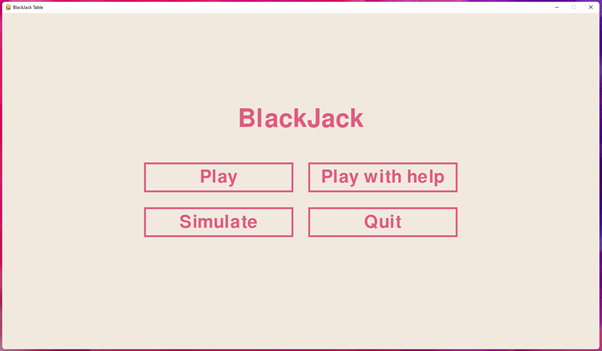
\includegraphics{meni.png}\,%
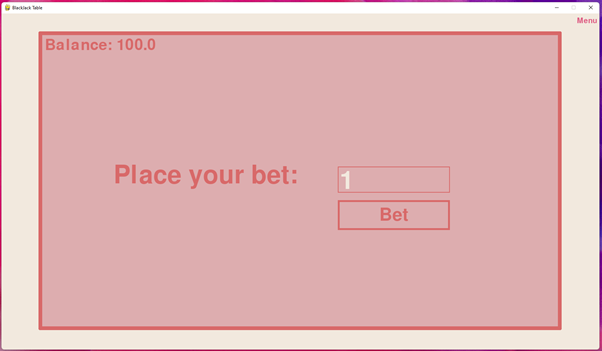
\includegraphics{bet.png}
  
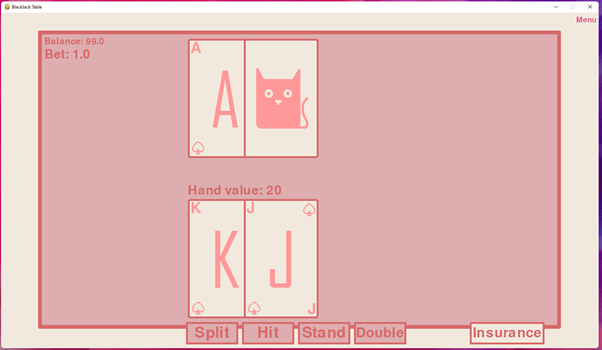
\includegraphics{table.png}\,%
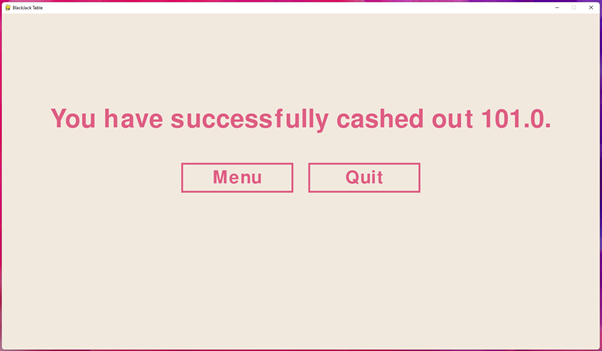
\includegraphics{cash_out.png}
\caption{Tako izgleda moja igra}
 \end{figure}

\noindent Poleg tega sem si tudi nastavila okolje za možnost igre s pomočjo. To pomeni, da bo igralec igral sam poleg hiši, vendar bo imel na voljo tudi verjetnosti katera akcija se mu bolj splača.\\

\noindent Del mojega programa na katerem trenutno delam je simulacijski del. Napisala sem že funkcije za sledeče strategije:
\begin{itemize}
\item Paroli system
\item 1 3 2 6 system
\item Reverse Labouchere
\item Martingale
\item Oscar’s Grind
\item Labouchere
\end{itemize}
Te so zbrane v mapi \textbf{functions} v datoteki \textbf{strategies.py}. Strategije so opisane \href{https://www.legitgamblingsites.com/blog/how-to-best-take-advantage-of-streaks-in-blackjack/}{tukaj.} Ob pravi uporaabi funkcij bo program stavljal po izbrani strategiji, njegove odločitve v določeni situaciji pa so že v naprej napisane in naj bi bile optimalne. 

 




\section{Še sledi}
\begin{itemize}
\item dokončati igro, kjer je navoljo pomoč
\item napisati funkcijo za računanje verjetnosti zmage v določeni situaciji
 \item dodati strategijo štetja kart
\item napisati funkcijo za hranjenje podatkov iz simulacije različnih strategij
\item analizirati dobljene podatke
\end{itemize}




\end{document}